\chapter{Theoretical Foundations}

This chapter provides the conceptual and methodological foundations for the thesis. It first reviews core deep learning principles that underlie modern neural text classification, including training dynamics, optimization, and generalization. It then introduces key definitions and conceptual distinctions from the misinformation literature that motivate computational detection settings. Building on this, the chapter summarizes transformer-based large language models and common adaptation strategies such as prompting and parameter-efficient fine-tuning. Finally, it introduces multi-agent 
systems in NLP as the architectural foundation for the multi-agent framework developed in subsequent chapters.

\section{Fundamentals of Deep Learning}

Deep learning is a subfield of machine learning based on artificial neural networks with multiple layers, enabling models to learn hierarchical representations of data. These models have achieved state-of-the-art performance across domains such as computer vision, natural language processing, and speech recognition, primarily due to advances in computational power, data availability, and optimization techniques \cite{RAZAVI2021105159}. The following subsections introduce feedforward networks, forward and backward propagation, common loss functions, and standard techniques for evaluation and regularization.

\subsection{Artificial Neurons and Neural Networks}

Artificial neural networks are inspired by biological neurons and consist of interconnected processing units called artificial neurons. Each neuron computes a weighted sum of its inputs, applies a nonlinear activation function, and produces an output signal. By stacking multiple layers of neurons, neural networks can model complex, non-linear relationships in data \cite{hammad2024artificialneuralnetworkdeep}. 

A typical neural network consists of an input layer, one or more hidden layers, and an output layer. The basic architecture of an artificial neural network is illustrated in Figure~\ref{fig:network3}. While shallow networks contain only a single hidden layer, deep neural networks include multiple hidden layers, allowing them to learn increasingly abstract representations. This hierarchical representation learning is a defining characteristic of deep learning and is critical for capturing semantic patterns in text data \cite{raghu2020surveydeeplearningscientific}.

\begin{figure}[htbp]
\centering
\begin{tikzpicture}[
    neuron/.style={circle, draw, fill=blue!80!black, text=white, 
                   minimum size=0.9cm, font=\small\bfseries},
    input/.style={font=\small},
    bias/.style={font=\small, text=green!60!black},
    arrow/.style={-{Stealth}, thick},
    label/.style={font=\footnotesize}
]

\node[input] (weight) at (0, 1.5) {weight};
\node[input] (height) at (0, -1.5) {height};

\node[neuron] (h1) at (5.0, 1.5) {$h_1$};
\node[neuron] (h2) at (5.0, -1.5) {$h_2$};

\node[bias] (b1) at (5.0, 2.6)  {$b_1$};
\node[bias] (b2) at (5.0, -0.4) {$b_2$};

\node[neuron] (o1) at (9.0, 0) {$o_1$};

\node[bias] (b3) at (9.8, 0.9) {$b_3$};

\node[font=\small\bfseries] at (0,   3.2) {Input Layer};
\node[font=\small\bfseries] at (5.0, 3.2) {Hidden Layer};
\node[font=\small\bfseries] at (9.0, 3.2) {Output Layer};

\node[font=\small] at (9.0, -1.1) {gender};

\draw[arrow] (weight.east) -- (h1.west) 
    node[near end, above, label] {$w_1$};
\draw[arrow] (weight.east) -- (h2.west) 
    node[near end, above right, label] {$w_3$};

\draw[arrow] (height.east) -- (h1.west) 
    node[near end, below right, label] {$w_2$};
\draw[arrow] (height.east) -- (h2.west) 
    node[near end, below, label] {$w_4$};

\draw[arrow] (h1.east) -- (o1.west) 
    node[near end, above, label] {$w_5$};
\draw[arrow] (h2.east) -- (o1.west) 
    node[near end, below, label] {$w_6$};

\draw[-{Stealth}, dashed, green!60!black] (b1) -- (h1);
\draw[-{Stealth}, dashed, green!60!black] (b2) -- (h2);
\draw[-{Stealth}, dashed, green!60!black] (b3) -- (o1);

\end{tikzpicture}
\caption{Architecture of a simple feedforward neural network with an input layer, a single hidden layer, and an output layer, illustrating weighted connections and bias terms.}
\label{fig:network3}
\end{figure}

In supervised learning, feedforward neural networks, often referred to as multilayer perceptrons (MLPs), are trained to approximate an unknown target function by learning a parameterized mapping $y \approx f_{\theta}(\mathbf{x})$ \cite{Goodfellow-et-al-2016}. This mapping is computed by successively applying linear transformations and nonlinear activation functions across layers. During training, the network adapts the parameters $\theta$ (weights and bias terms) to minimize the discrepancy between its predictions and the ground-truth targets. This discrepancy is quantified by a loss function, which provides the objective for optimization. The following subsection introduces forward propagation and the associated loss computation.


\subsection{Forward Propagation and Loss Computation}

Forward propagation refers to the process of passing input data through the network layer by layer to generate a prediction \cite{zhang2023dive}. At each layer, neurons apply affine transformations followed by nonlinear activation functions, enabling the network to model complex mappings between inputs and outputs.

Given an input vector $\mathbf{x} = (x_1, x_2)$, each hidden neuron computes a weighted sum of the inputs followed by a nonlinear activation function $\sigma(\cdot)$. Common activation functions include the Rectified Linear Unit (ReLU), the hyperbolic tangent, and the sigmoid, as illustrated in Figure~\ref{fig:activation_functions}. The output neuron applies a further linear transformation and activation function to produce the network prediction $\hat{y} \in (0,1)$.

    \begin{figure}[htbp]
        \centering
        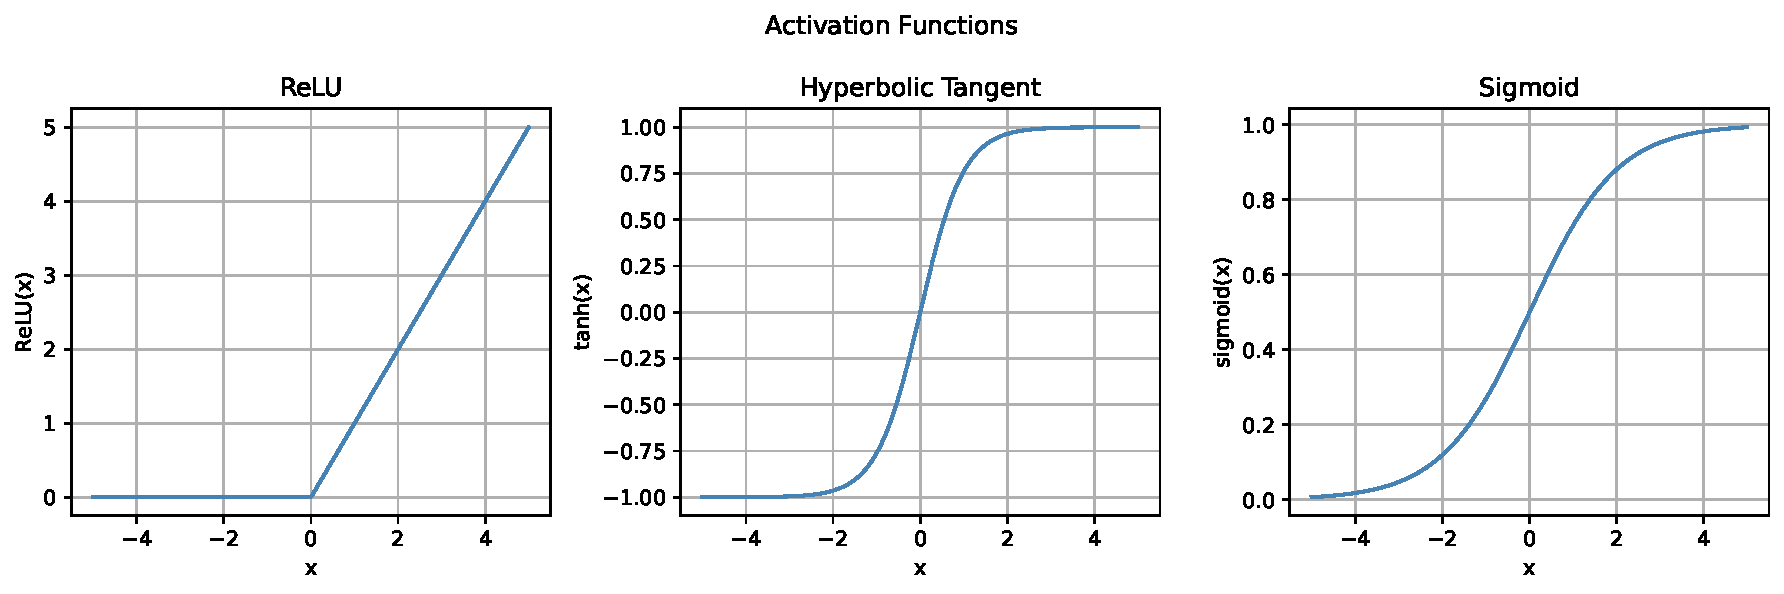
\includegraphics[width=0.9\textwidth]{Bilder/activation_functions.pdf}
        \caption{Common activation functions used in neural networks: ReLU, Hyperbolic Tangent (tanh), and Sigmoid \cite{activation}.}
        \label{fig:activation_functions}
    \end{figure}
\FloatBarrier

The sigmoid activation function $\sigma(\cdot)$ is defined as
\begin{equation}
\sigma(z) = \frac{1}{1+e^{-z}}.
\end{equation}

The forward pass proceeds in two stages. In the hidden layer, pre-activations $z_{h_1}$ and $z_{h_2}$ are computed as affine transformations of the input and mapped to activations $h_1$ and $h_2$ using $\sigma(\cdot)$. The output layer then computes $z_o$ from $h_1$ and $h_2$, and applying $\sigma(\cdot)$ yields the prediction $\hat{y} \in (0,1)$. All weights $\{w_i\}$ and bias terms $\{b_i\}$ are learned by minimizing a loss function.

\begin{align}
z_{h_1} &= w_1 x_1 + w_2 x_2 + b_1, & h_1 &= \sigma(z_{h_1}) \\
z_{h_2} &= w_3 x_1 + w_4 x_2 + b_2, & h_2 &= \sigma(z_{h_2}) \\
z_o &= w_5 h_1 + w_6 h_2 + b_3, & \hat{y} &= \sigma(z_o)
\end{align}

The quality of a prediction is measured using a loss function, which quantifies the discrepancy between the predicted output and the true target. 

\begin{equation}
\mathcal{L}_{\mathrm{BCE}}(y,\hat{y}) = -\left[y \log(\hat{y}) + (1-y)\log(1-\hat{y})\right].
\label{eq:bce}
\end{equation}

\begin{equation}
\mathcal{L}_{\mathrm{MSE}}(y,\hat{y}) = \frac{1}{2}\,(y-\hat{y})^2.
\label{eq:mse}
\end{equation}

Common loss functions include binary cross-entropy (BCE) loss defined in Equation~\eqref{eq:bce} for classification tasks and mean squared error for regression problems defined in Equation~\eqref{eq:mse}. The loss function provides the optimization objective that guides the learning process \cite{elharrouss2025taskbasedlossfunctionscomputer}.
This forward propagation process defines a differentiable mapping from inputs to outputs, enabling the network parameters to be optimized via gradient-based learning methods. In the binary classification setting with a sigmoid output, combining the BCE loss with $\hat{y}=\sigma(z_o)$ yields a particularly simple gradient expression that is used in the backpropagation derivation.

\subsection{Backpropagation and Gradient-Based Optimization}

Backpropagation is the core algorithm used to train neural networks. It computes gradients of the loss function with respect to all model parameters by recursively applying the chain rule in a backward pass through the network. These gradients indicate how each parameter should be adjusted in order to minimize the loss function \cite{RAZAVI2021105159}.

The derivative of the sigmoid activation function is given by
\begin{equation}
\sigma'(z) = \sigma(z)\bigl(1-\sigma(z)\bigr).
\end{equation}

For the output layer, the error term is defined as the derivative of the loss with respect to the pre-activation value $z_o$. When using a sigmoid activation function in combination with the binary cross-entropy loss, this term simplifies to
\begin{equation}
\delta_o \;\triangleq\; \frac{\partial \mathcal{L}}{\partial z_o}
= \hat{y} - y.
\end{equation}

The error terms for the hidden layer neurons are obtained by propagating the output error backward through the network:
\begin{align}
\delta_{h_1} &= (w_5 \delta_o)\, \sigma'(z_{h_1})
= (w_5 \delta_o)\, h_1(1-h_1), \\
\delta_{h_2} &= (w_6 \delta_o)\, \sigma'(z_{h_2})
= (w_6 \delta_o)\, h_2(1-h_2).
\end{align}

Using these error terms, the gradients of the loss function with respect to the network parameters can be computed as
\begin{align}
\frac{\partial \mathcal{L}}{\partial w_1} &= \delta_{h_1} \, x_1, &
\frac{\partial \mathcal{L}}{\partial w_2} &= \delta_{h_1} \, x_2, &
\frac{\partial \mathcal{L}}{\partial b_1} &= \delta_{h_1}, \\
\frac{\partial \mathcal{L}}{\partial w_3} &= \delta_{h_2} \, x_1, &
\frac{\partial \mathcal{L}}{\partial w_4} &= \delta_{h_2} \, x_2, &
\frac{\partial \mathcal{L}}{\partial b_2} &= \delta_{h_2}, \\
\frac{\partial \mathcal{L}}{\partial w_5} &= \delta_o \, h_1, &
\frac{\partial \mathcal{L}}{\partial w_6} &= \delta_o \, h_2, &
\frac{\partial \mathcal{L}}{\partial b_3} &= \delta_o.
\end{align}

Model parameters are updated iteratively using gradient-based optimization methods. In its simplest form, gradient descent updates each parameter $\theta$ according to
\begin{equation}
\theta \leftarrow \theta - \eta \frac{\partial \mathcal{L}}{\partial \theta},
\end{equation}
where $\eta$ denotes the learning rate. More advanced optimization algorithms, such as stochastic gradient descent with momentum, Adam, or RMSProp, adapt the learning rate dynamically to improve convergence speed and training stability, particularly in deeper network architectures \cite{sun2019optimizationdeeplearningtheory}.

In deep networks, gradients can vanish or explode as they are propagated through many layers. This effect is amplified by saturating activation functions such as the sigmoid, whose derivative becomes close to zero for large positive or negative inputs, slowing learning in earlier layers. Common mitigation strategies include non-saturating activations (e.g., ReLU), careful initialization, normalization methods, and gradient clipping \cite{elharrouss2025taskbasedlossfunctionscomputer}.

\subsection{Model Training and Evaluation}

Model training involves iteratively updating network parameters using labeled training data until convergence or until a predefined stopping criterion is met. To assess model performance and generalization capability, datasets are commonly divided into training, validation, and test sets.

Training is typically performed over multiple \emph{epochs}, where one epoch corresponds to a full pass over the training dataset. Parameters are updated in \emph{iterations} (or steps), commonly using \emph{mini-batches} of size $B$ rather than the full dataset to reduce computational cost and to obtain more frequent updates. This yields stochastic or mini-batch gradient descent updates, 
which are the standard training regime for modern neural networks \cite{hammad2024artificialneuralnetworkdeep}.

Evaluation metrics depend on the specific task and provide quantitative measures of model performance. For binary classification problems, commonly used metrics include accuracy, precision, recall, and the F1-score, which are derived from the confusion matrix consisting of true positives (TP), true negatives (TN), false positives (FP), and false negatives (FN). Figure~\ref{fig:confusion_matrix} illustrates the confusion matrix structure and the corresponding metric definitions, with color coding indicating which cells contribute to each metric.

\begin{figure}[htbp]
\centering
\begin{tikzpicture}[
    cell/.style={rectangle, minimum width=2.8cm, minimum height=1.8cm, 
                 draw, align=center, font=\small},
]

\node[font=\small\bfseries] at (5.7, 3.8) {Predicted Label};
\node[font=\small, align=center] at (4.3, 3.1) {Predicted\\True};
\node[font=\small, align=center] at (7.1, 3.1) {Predicted\\False};

\node[font=\small\bfseries, rotate=90] at (0.0, 0.7) {Actual Label};
\node[font=\small, align=center, rotate=90] at (1.2, 1.6) {Actual\\True};
\node[font=\small, align=center, rotate=90] at (1.2, -0.2) {Actual\\False};

\node[cell, fill=green!25] (TP) at (4.3, 1.6) {
    \textbf{TP}\\
    \footnotesize True Positive\\
    \footnotesize (correct)};

\node[cell, fill=red!20] (FN) at (7.1, 1.6) {
    \textbf{FN}\\
    \footnotesize False Negative\\
    \footnotesize (missed)};

\node[cell, fill=orange!25] (FP) at (4.3, -0.2) {
    \textbf{FP}\\
    \footnotesize False Positive\\
    \footnotesize (false alarm)};

\node[cell, fill=green!25] (TN) at (7.1, -0.2) {
    \textbf{TN}\\
    \footnotesize True Negative\\
    \footnotesize (correct)};

\node[align=left, font=\small] at (12.5, 2.4) {
    $\mathrm{Accuracy} = \dfrac{
        \textcolor{green!60!black}{\mathbf{TP}} + 
        \textcolor{green!60!black}{\mathbf{TN}}}{
        \textcolor{green!60!black}{\mathbf{TP}} + 
        \textcolor{green!60!black}{\mathbf{TN}} + 
        \textcolor{orange!80!black}{\mathbf{FP}} + 
        \textcolor{red!70!black}{\mathbf{FN}}}$};

\node[align=left, font=\small] at (12.5, 1.1) {
    $\mathrm{Precision} = \dfrac{
        \textcolor{green!60!black}{\mathbf{TP}}}{
        \textcolor{green!60!black}{\mathbf{TP}} + 
        \textcolor{orange!80!black}{\mathbf{FP}}}$};

\node[align=left, font=\small] at (12.5, -0.2) {
    $\mathrm{Recall} = \dfrac{
        \textcolor{green!60!black}{\mathbf{TP}}}{
        \textcolor{green!60!black}{\mathbf{TP}} + 
        \textcolor{red!70!black}{\mathbf{FN}}}$};

\node[align=left, font=\small] at (12.5, -1.4) {
    $\mathrm{F1} = 2 \cdot \dfrac{
        \mathrm{Precision} \cdot \mathrm{Recall}}{
        \mathrm{Precision} + \mathrm{Recall}}$};

\draw[dashed, gray] (9.0, -1.8) -- (9.0, 4.0);

\end{tikzpicture}
\caption{Confusion matrix for binary classification and derived evaluation metrics. \textcolor{green!60!black}{\textbf{TP}} and \textcolor{green!60!black}{\textbf{TN}} denote correct predictions; \textcolor{orange!80!black}{\textbf{FP}} and 
\textcolor{red!70!black}{\textbf{FN}} denote incorrect predictions.}
\label{fig:confusion_matrix}
\end{figure}

Proper evaluation using these metrics is essential for identifying overfitting, detecting potential biases in the data, and comparing alternative model architectures or training strategies \cite{raghu2020surveydeeplearningscientific}.

\subsection{Regularization Techniques}

Regularization techniques are used to prevent overfitting and improve generalization. Common approaches include L1 and L2 weight regularization, which penalize large parameter values, and dropout, which randomly disables neurons during training to encourage redundancy and robustness.

Early stopping is another effective regularization method, where training is halted once performance on a validation set stops improving. These techniques help neural networks generalize better to unseen data, especially when training data is limited or noisy \cite{hammad2024artificialneuralnetworkdeep}.

\subsection{Normalization Methods}

Normalization methods stabilize and accelerate training by reducing internal covariate shift. Feature scaling techniques such as normalization and standardization ensure that input features have comparable scales.

Batch normalization extends this idea to hidden layers by normalizing intermediate activations during training. This technique improves gradient flow, allows higher learning rates, and reduces sensitivity to parameter initialization, making deep networks easier to train \cite{RAZAVI2021105159}.

\subsection{Overfitting and Generalization}

Overfitting occurs when a model learns patterns specific to the training data that do not generalize to unseen data \cite{valdenegrotoro2022machinelearningstudentsoverfit}. This issue is particularly severe in high-capacity models trained on limited datasets.

Generalization refers to a model’s ability to perform well on new data drawn from the same or similar distributions. Achieving good generalization requires appropriate model complexity, sufficient data diversity, and effective regularization strategies. Understanding this trade-off is critical when applying deep learning models to real-world tasks such as fake news detection, where data distributions may shift over time \cite{raghu2020surveydeeplearningscientific}.

\section{Fake News and Detection}

Fake news detection is closely related to fact-checking, misinformation studies, and computational credibility assessment. While fact-checking typically focuses on verifying the truthfulness of individual claims (often short statements), fake news detection often targets longer pieces of content such as full articles or posts and aims to assess their overall trustworthiness \cite{vykopal2024generativelargelanguagemodels}. The following subsections introduce key definitions, taxonomies, and conceptual properties that are commonly used to frame fake news and its automated detection.

\subsection{Definitions and Taxonomies}

The term \emph{fake news} does not have a universally agreed definition, partly because its meaning has changed over time and it is often used rhetorically as a political label to discredit opponents. In academic contexts, definitions frequently converge on three criteria: (i) the content is false or misleading, (ii) it is presented in a news-like format, and (iii) it serves a deceptive or misleading function, even though the role of intent is debated \cite{encyclopedia2010043}. A widely used operational definition describes fake news as news-like content that is intentionally false or misleading and designed to deceive \cite{fi16080298}.

Taxonomies further distinguish different forms of fake news and related deceptive content. One common categorization includes political propaganda, fabricated stories, manipulated content (e.g., real events presented out of context), and parody or satire \cite{10704605}. Importantly, fake news is increasingly treated as a subtype of online disinformation that imitates journalistic conventions while violating epistemic and professional standards such as verification and accountability \cite{encyclopedia2010043}. These taxonomies emphasize that fake news is not a single phenomenon but a spectrum of deceptive practices that vary in their goals, presentation strategies, and modes of dissemination.

\subsection{Structure of Deceptive Content}

Fake news is often effective because it imitates the structure and appearance of legitimate journalism. This imitation can operate at multiple levels, including textual style (e.g., headline conventions and narrative flow), visual presentation (e.g. images, layout, or logos), and platform embedding (e.g., how items appear in feeds or previews). Structural similarity to real news tends to increase perceived credibility and can support wider diffusion \cite{appel-2019}.

Deception also frequently arises from \emph{composition} rather than pure fabrication. Many instances combine fabricated claims, distorted facts, half-truths, and even literally true statements placed in misleading contexts. Misleading meaning can be produced through framing, selective ordering of information, or omission of crucial context \cite{encyclopedia2010043}. As a result, fake news may be difficult to detect using purely surface-level cues, since credible structure and partially accurate content can mask deeper forms of manipulation.

\subsection{Misinformation vs. Disinformation}

A central distinction in the literature separates misinformation from disinformation. Misinformation refers to false or inaccurate information shared without intent to deceive, often caused by mistakes, negligence, or misunderstandings \cite{10704605}. Disinformation, in contrast, is intentionally false information created and disseminated to mislead, manipulate, or cause harm, and is often associated with political propaganda \cite{10704605,fi16080298}.

Fake news overlaps strongly with disinformation but cannot always be reduced to deliberate lying. Some creators may be largely indifferent to truth and primarily motivated by attention, virality, or profit (e.g., click-driven content), which complicates intent-based definitions. This distinction is especially important for automated detection systems: intent is rarely observable from text alone, and reliable intent inference is generally not feasible at scale. Consequently, practical computational definitions often focus on observable properties such as verifiability, evidentiary grounding, and violations of journalistic norms rather than psychological intent \cite{encyclopedia2010043}.

\subsection{Domain Dependence in Classification}

Fake news is highly context- and domain-dependent. Deceptive strategies, expected evidence standards, and persuasive rhetoric differ substantially across domains such as politics, public health, science, and commerce \cite{encyclopedia2010043,tong-etal-2025-generate}. In addition, the same content may be misleading for one audience but not for another, because interpretation depends on background knowledge, cultural context, and platform-specific presentation \cite{encyclopedia2010043}.

This domain dependence creates major challenges for classification systems. Models trained on one dataset or domain often exploit domain-specific cues and may fail when deployed on new topics or domains, leading to weak cross-domain generalization \cite{tong-etal-2025-generate}. Prior work has therefore explored incorporating social context (e.g., comment-reply structures and propagation patterns) and integrating external knowledge to improve robustness, although these enhancements may require additional data collection effort and system complexity \cite{tong-etal-2025-generate}. Overall, domain dependence motivates domain-aware modeling strategies and evaluation protocols that explicitly test generalization beyond the training distribution.

\subsection{Linguistic and Contextual Properties}

Linguistic analyses frequently associate fake news with sensationalism, emotional and polarized language, exaggeration, and strong certainty markers \cite{encyclopedia2010043,10704605}. However, such features are not reliable in isolation. High-quality fake news can be written in a professional tone and closely resemble legitimate reporting, while real news—especially in early reporting phases—may contain uncertainty or incomplete information \cite{encyclopedia2010043}.

Context is often decisive for deception. Misleading meaning can arise even when individual sentences are factually correct, for example when facts are selectively presented, crucial information is omitted, or content is framed to imply unsupported conclusions \cite{encyclopedia2010043}. This implies that effective detection should not be limited to sentence-level signals. Instead, models must capture discourse-level structure, pragmatic framing, and the relationship between claims and the contexts in which they are presented.

\subsection{Conceptualizing Lies in Computational Terms}

In philosophical terms, lying presupposes both knowledge of the truth and an intention to deceive. Translating this notion into automated detection is difficult because machine learning systems have no access to mental states and cannot directly observe intent \cite{encyclopedia2010043}. As a result, computational work typically reframes deception as an observable divergence from verifiable reality or from journalistic and epistemic norms.

Within fake news research, three common computational formulations can be distinguished. First, \emph{classification} assigns categorical labels (e.g., fake vs. real). Second, \emph{verification} evaluates claims against evidence, aligning closely with fact-checking pipelines. Third, \emph{credibility estimation} ranks or scores content according to trustworthiness. Recent progress in large language models has influenced all three formulations: generative models can produce richer outputs such as explanations, reasoning traces, and claim decomposition, which may improve interpretability. At the same time, LLMs may hallucinate, misinterpret claims, or provide incorrect justifications, and they may lack up-to-date knowledge without external retrieval \cite{vykopal2024generativelargelanguagemodels}.

\section{Large Language Models and Transformers}

Large language models have emerged as a dominant paradigm in natural language processing, enabling strong performance across a wide range of tasks without task-specific architectures. Their success is largely driven by advances in transformer-based architectures, large-scale pretraining, and flexible adaptation strategies such as prompting and fine-tuning. This section introduces the theoretical foundations of LLMs, focusing on their architectural components, training paradigms, and usage patterns that are relevant for fake news detection.

\subsection{Evolution of NLP Models}

Natural language processing has progressed alongside a broader change in AI: from hand-built linguistic systems to models that learn language patterns from data at scale. Early NLP work (roughly the 1950s–1970s) was dominated by symbolic and rule-based approaches. These systems relied on manually crafted grammars, pattern matching, and logic-based representations to parse text, translate sentences, or imitate dialogue (e.g., early machine translation efforts and ELIZA). While transparent and easy to interpret, rule-based systems struggled with ambiguity and variation in real-world language and did not generalize well beyond the scenarios anticipated by their designers \cite{chen2025deeplearningmachinelearning}.

Beginning in the 1980s, the field increasingly adopted probabilistic and statistical techniques to overcome these limitations. Classic statistical language models—especially n-gram models—estimated word probabilities from corpus statistics but were limited by short context windows and strong independence assumptions \cite{zhao2025surveylargelanguagemodels}. Even when effective for narrow tasks, these models suffered from sparsity and could not capture long-range dependencies reliably. During the 1990s, supervised machine learning further expanded NLP capabilities, supported by larger datasets and the growing availability of labeled corpora \cite{chen2025deeplearningmachinelearning}.

A major shift occurred in the 2010s with neural language models. Distributed representations (word embeddings) and end-to-end learning enabled models to capture linguistic regularities directly from data. Sequence models such as RNNs and LSTMs improved the ability to represent contextual dependencies, but they remained difficult to parallelize and scale efficiently. Transformer architectures changed this by replacing recurrence with attention, allowing much larger models to be trained effectively \cite{chen2025deeplearningmachinelearning}.

This development led to the pretraining paradigm that dominates modern NLP: large-scale self-supervised learning on general text, followed by task adaptation through fine-tuning or prompting. Large language models extend this approach by further increasing model capacity and training data, yielding strong zero-shot and few-shot performance across many tasks. As a result, NLP has shifted away from building separate task-specific systems and toward general-purpose models that can be adapted across domains with minimal additional supervision \cite{zhao2025surveylargelanguagemodels}.

\subsection{Transformer Architecture and Attention Mechanisms}

The Transformer architecture forms the foundation of modern large language models, including the LLaMA family used in this thesis. Unlike recurrent or convolutional architectures, transformers process entire token sequences in parallel, enabling efficient training and scalability to very large datasets \cite{vaswani2023attentionneed}.

A transformer layer consists of two main components: a multi-head self-attention mechanism and a position-wise feed-forward network. These components are combined with residual connections and layer normalization to stabilize training and enable deep architectures \cite{vaswani2023attentionneed}. By stacking multiple such layers, transformers can model complex, long-range dependencies within text, which is essential for reasoning-intensive tasks \cite{naveed2024comprehensiveoverviewlargelanguage}. Figure~\ref{fig:transformer-architecture} shows the original encoder--decoder Transformer architecture. The encoder (left) and decoder (right) are each composed of \(N\) stacked layers, where each layer combines multi-head attention and a position-wise feed-forward network, wrapped with residual connections and layer normalization (``Add \& Norm''). The decoder applies masked self-attention so that each token can only use information from earlier tokens, then uses encoder--decoder attention to incorporate the encoder representations, and finally outputs token probabilities via a linear layer and a softmax.

\begin{figure}[htbp]
    \centering
    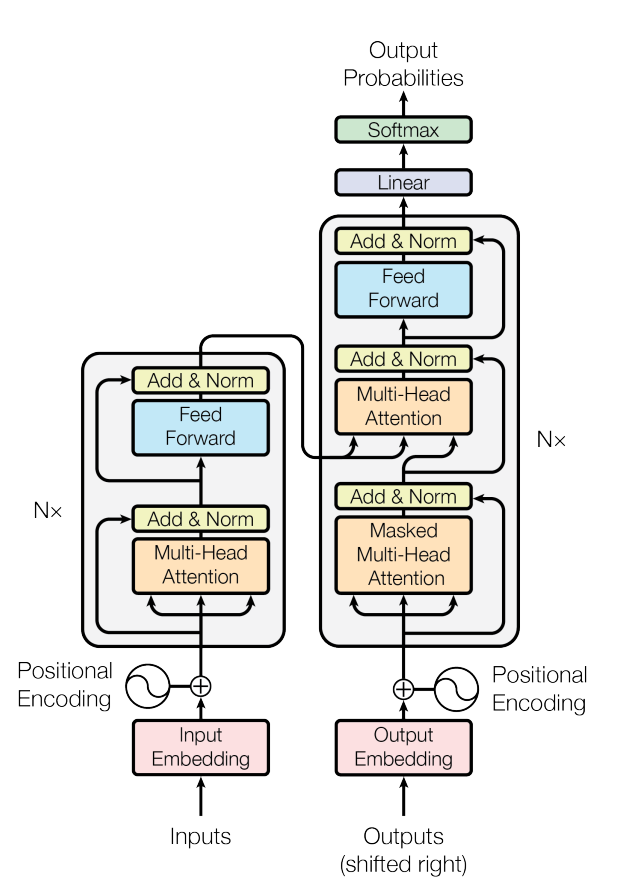
\includegraphics[width=0.4\textwidth]{Bilder/Transformer.png}
    \caption{Transformer model architecture (encoder–decoder) with the encoder shown on the left and the decoder on the right, as introduced by Vaswani et al.~\cite{vaswani2023attentionneed}.}
    \label{fig:transformer-architecture}
\end{figure}

Self-attention allows each token to attend to all other tokens in the sequence, weighting their relevance dynamically based on learned similarity scores \cite{vaswani2023attentionneed}. This enables the model to integrate contextual information regardless of token distance. Figure~\ref{fig:self_attention} illustrates the scaled dot-product self-attention computation for a single head. The input token embeddings \(X\) (here shown for the tokens \emph{``I''}, \emph{``love''}, \emph{``tennis''}) are linearly projected using learned weight matrices \(W_Q\), \(W_K\), and \(W_V\) to form queries \(Q=XW_Q\), keys \(K=XW_K\), and values \(V=XW_V\). Attention scores are computed as \(QK^\top/\sqrt{d_k}\) and normalized with a softmax to obtain the attention weight matrix \(S\). Multiplying these weights with the values (\(SV\)) produces the attention output, i.e. context-aware token embeddings where each token aggregates information from other tokens according to its learned relevance weights.

Multi-head attention extends this mechanism by computing several attention distributions in parallel, allowing the model to capture different types of relationships, such as syntactic structure or semantic relevance, within the same layer \cite{devlin2019bertpretrainingdeepbidirectional}.

\begin{figure}[htbp]
    \centering
    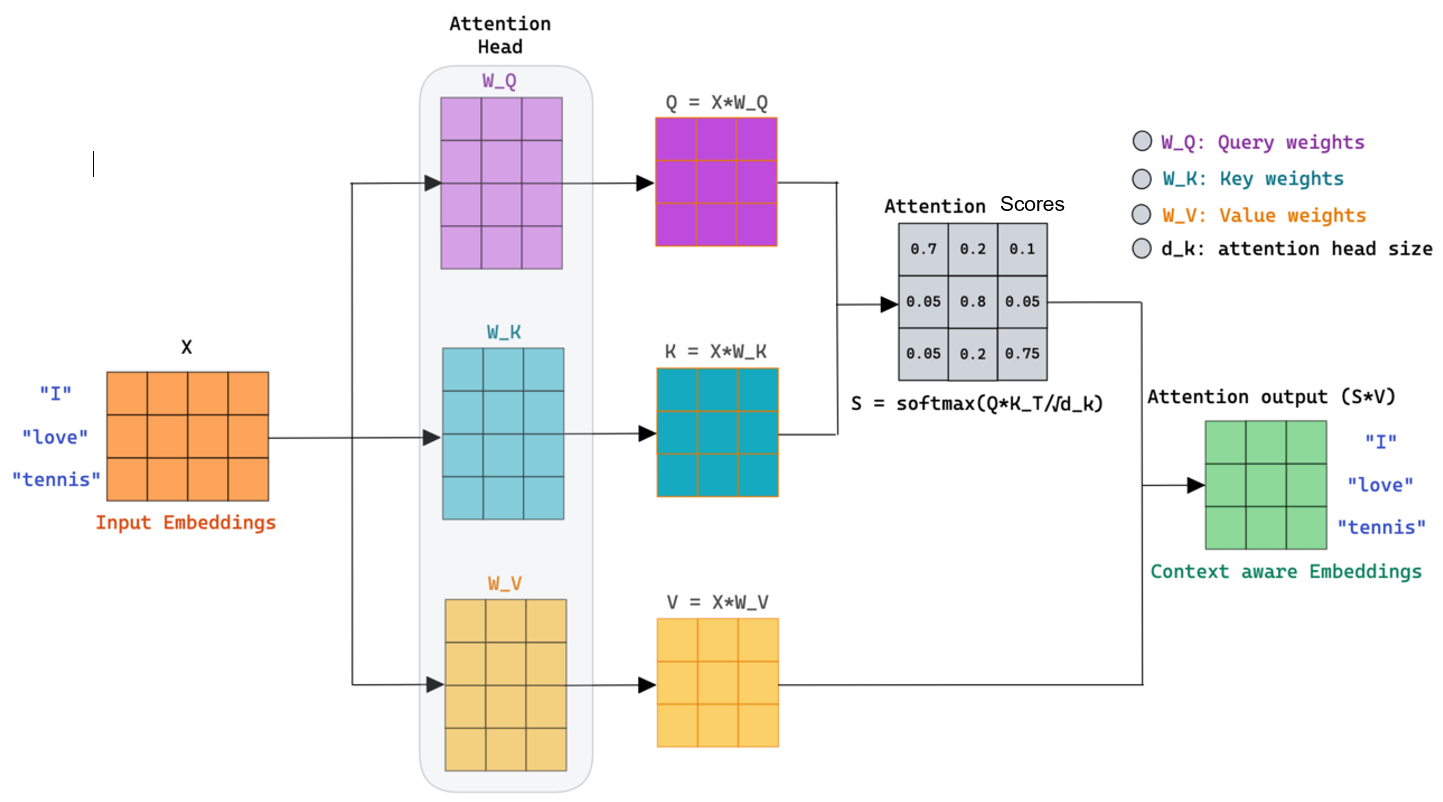
\includegraphics[width=0.9\textwidth]{Bilder/self_attention_thumbnail_corrected.png}
    \caption{Scaled dot-product self-attention (single head). Multi-head attention repeats this computation in parallel across multiple heads and concatenates the results \cite{pachaar-2025}.}
    \label{fig:self_attention}
\end{figure}

Because transformers process tokens simultaneously, they do not inherently encode word order. Positional information is therefore injected into the model using positional encodings \cite{vaswani2023attentionneed}. These encodings enable the model to distinguish between different token positions and to capture sequential structure, which is critical for tasks involving logical flow, temporal relations, or argument structure \cite{naveed2024comprehensiveoverviewlargelanguage}.

Decoder-only transformer models, such as LLaMA, employ causal self-attention masks that restrict each token to attending only to previous tokens in the sequence \cite{brown2020languagemodelsfewshotlearners}. This design supports autoregressive generation and allows the same architecture to be used for both input conditioning and output generation. Due to their architectural simplicity and strong performance in prompt-based settings, decoder-only transformers have become the dominant architecture for large language models \cite{touvron2023llamaopenefficientfoundation}.

\subsection{Tokenization and Embeddings}

Before text can be processed by a transformer, it must be converted into a sequence of tokens. Modern LLMs typically rely on subword tokenization methods, such as Byte Pair Encoding or related variants, which balance vocabulary size and expressiveness while mitigating out-of-vocabulary issues \cite{chen2025deeplearningmachinelearning}.

Each token is mapped to a continuous vector representation, known as an embedding. These embeddings serve as the initial input to the transformer and are learned during training \cite{chen2025deeplearningmachinelearning}. Embeddings enable the model to represent semantic and syntactic relationships between tokens in a continuous space, forming the basis for higher-level language understanding.

\subsection{Encoder--Decoder vs. Decoder-Only Models}

Transformer-based models can be broadly categorized into encoder--decoder architectures and decoder-only architectures. Encoder--decoder models consist of separate encoder and decoder components, where the encoder processes the input sequence and the decoder generates the output conditioned on the encoder representation. This architecture is commonly used for sequence-to-sequence tasks such as translation \cite{zhao2025surveylargelanguagemodels}.

Decoder-only models, in contrast, use a single transformer stack with causal attention masks, enabling autoregressive text generation. This architecture underlies most modern large language models and has demonstrated strong performance in zero-shot and few-shot settings \cite{naveed2024comprehensiveoverviewlargelanguage}. Decoder-only models are particularly relevant for prompt-based fake news detection, as both input and output can be handled within a single model.

\subsection{Representative LLM Families}

Several families of large language models have been proposed, differing in architecture, training strategy, and scale. Examples include instruction-tuned models, multilingual models, and mixture-of-experts architectures that activate only a subset of parameters during inference \cite{naveed2024comprehensiveoverviewlargelanguage}. These design choices aim to balance performance, efficiency, and generalization.

Despite architectural differences, most LLMs share a common foundation: transformer-based modeling, large-scale pretraining on diverse text corpora, and adaptation through prompting or fine-tuning. These shared characteristics enable comparative evaluation across models in downstream tasks such as fake news detection.

\subsection{Pretraining and Fine-Tuning Paradigms}

Large language models are typically pretrained using self-supervised objectives on large unlabeled text corpora, allowing them to acquire broad linguistic and world knowledge without task-specific supervision \cite{zhao2025surveylargelanguagemodels}. Since pretraining on billions of tokens is prohibitively expensive, the dominant paradigm reuses these pretrained weights and adapts them to downstream tasks through fine-tuning -- a second training phase on smaller, task-specific labeled datasets \cite{naveed2024comprehensiveoverviewlargelanguage}. This two-stage approach combines the broad generalization of pretraining with the precision of task-specific supervision.

\paragraph{Supervised Fine-Tuning (SFT).}
Supervised fine-tuning (SFT) is the most direct form of task adaptation. Given a labeled dataset of input--output pairs, the model is trained to minimize a task-specific loss, typically cross-entropy over the target tokens. In instruction-following settings, inputs are formatted as natural language prompts and outputs as expected completions, encouraging the model to follow instructions reliably \cite{zhao2025surveylargelanguagemodels}. SFT has been shown to substantially improve task-specific performance compared to zero-shot prompting, particularly for classification tasks with well-defined output formats.

\paragraph{Instruction Fine-Tuning.}
Instruction fine-tuning extends SFT by training on a diverse mixture of tasks formatted as natural language instructions. This approach improves generalization to unseen tasks and enhances instruction-following behavior across domains \cite{naveed2024comprehensiveoverviewlargelanguage}. Models trained with instruction fine-tuning, such as FLAN-T5 and LLaMA-Instruct variants, are better aligned with user intent and typically outperform base models in zero-shot and few-shot settings.

\paragraph{Domain-Specific Fine-Tuning.}
Beyond general task adaptation, fine-tuning can be applied to specific topical domains by restricting the training data to domain-relevant examples. Domain-specific fine-tuning allows models to learn domain-specific patterns, terminology, and label distributions that may not be well represented in general pretraining corpora \cite{lu2024finetuninglargelanguagemodels}. However, this specialization can reduce generalization to out-of-domain examples, creating a trade-off between in-domain performance and cross-domain robustness that must be carefully managed through evaluation on held-out distributions.

\paragraph{Completion-Only Training.}
In practice, fine-tuning for classification or constrained generation tasks is often implemented in a completion-only style: the model receives a formatted prompt and is trained to generate only the target label or output, while prompt tokens are masked out in the loss computation. This approach focuses optimization on the decision-relevant part of the output and avoids the model wasting capacity on reproducing the input \cite{naveed2024comprehensiveoverviewlargelanguage}.

\subsection{Parameter-Efficient Fine-Tuning with LoRA}

Fine-tuning large language models typically requires updating all model parameters, which becomes increasingly infeasible as model sizes grow. For a model such as GPT-3 with 175 billion parameters, storing and deploying separate fine-tuned instances for each downstream task is prohibitively expensive \cite{hu2021loralowrankadaptationlarge}.

Parameter-efficient fine-tuning methods address this limitation by adapting only a small subset of parameters while keeping the base model frozen. Low-Rank Adaptation (LoRA) is one such approach, proposed by Hu et al. \cite{hu2021loralowrankadaptationlarge}. The key insight behind LoRA is that the weight updates during fine-tuning have a low intrinsic rank -- that is, the change in weights $\Delta W$ can be well approximated by a low-rank decomposition.

\paragraph{Core mechanism.}
Instead of directly updating a weight matrix $W \in \mathbb{R}^{d \times d}$, LoRA freezes $W$ and injects two trainable low-rank matrices $A \in \mathbb{R}^{d \times r}$ and $B \in \mathbb{R}^{r \times d}$, where the rank $r \ll d$. The modified forward pass computes:

\begin{equation}
h = Wx + \Delta Wx = Wx + BAx,
\end{equation}

where $x$ is the input and $\Delta W = BA$ approximates the weight update. Matrix $A$ is initialized with a random Gaussian distribution and $B$ is initialized to zero, ensuring that $\Delta W = 0$ at the start of training and the model begins from the pretrained state \cite{hu2021loralowrankadaptationlarge}.

Figure~\ref{fig:lora} illustrates this reparametrization. The pretrained weights $W$ remain frozen throughout training, while only the small matrices $A$ and $B$ are updated. The number of trainable parameters is reduced from $d \times d$ to $r \times (d + d) = 2rd$, which for typical values of $r \in \{4, 8, 16\}$ and $d$ in the thousands represents a reduction of several orders of magnitude.

\begin{figure}[htbp]
\centering
\begin{tikzpicture}[
    box/.style={rectangle, rounded corners=3pt, draw, minimum width=2.0cm,
                minimum height=1.0cm, align=center, font=\small},
    frozen/.style={box, fill=gray!20, draw=gray!60},
    trainable/.style={box, fill=blue!20, draw=blue!60},
    arrow/.style={-{Stealth}, thick},
]

\node[font=\small\bfseries] at (1.5, 4.0) {Full Fine-Tuning};
\node (x_left) at (-0.3, 2.0) {$x$};
\node[frozen] (W_full) at (1.5, 2.0) {$W + \Delta W$\\\footnotesize $d \times d$};
\node (h_left) at (3.3, 2.0) {$h$};
\node[font=\footnotesize, text=red!70!black, align=center] at (1.5, 0.6) 
    {all parameters\\updated};

\draw[arrow] (x_left) -- (W_full);
\draw[arrow] (W_full) -- (h_left);

\draw[dashed, gray] (4.0, -0.8) -- (4.0, 4.5);

\node[font=\small\bfseries] at (8.0, 4.0) {LoRA};

\node (x_right) at (4.7, 2.0) {$x$};

\node[frozen, minimum width=3.0cm] (W) at (8.0, 2.8) {$W$\\\footnotesize frozen};

\node[trainable] (A) at (6.5, 0.8) {$A$\\\footnotesize $d \times r$};
\node[trainable] (B) at (9.3, 0.8) {$B$\\\footnotesize $r \times d$};

\node[font=\small, circle, draw, inner sep=1pt] (plus) at (11.0, 2.0) {$+$};
\node (h_right) at (12.3, 2.0) {$h$};

\node[font=\footnotesize, text=blue!70!black, align=center] at (8.5, -0.5) 
    {only $A$, $B$ updated\\$r \ll d$};

\draw[arrow] (x_right) |- (W.west);

\draw[arrow] (x_right) |- (A.west);

\draw[arrow] (A) -- (B);

\draw[arrow] (W.east) -| (plus.north);

\draw[arrow] (B.east) -| (plus.south);

\draw[arrow] (plus) -- (h_right);

\end{tikzpicture}
\caption{Comparison of full fine-tuning and LoRA. In full fine-tuning, all 
parameters of $W$ are updated. In LoRA, $W$ is frozen and only the low-rank 
matrices $A \in \mathbb{R}^{d \times r}$ and $B \in \mathbb{R}^{r \times d}$ 
are trained, where $r \ll d$. The weight update is approximated as 
$\Delta W = BA$ \cite{hu2021loralowrankadaptationlarge}.}
\label{fig:lora}
\end{figure}

\paragraph{Advantages.}
LoRA offers several practical benefits \cite{hu2021loralowrankadaptationlarge}:
\begin{itemize}
    \item \textbf{Storage efficiency:} Multiple task-specific adapters can share 
    a single frozen base model, with only the small $A$ and $B$ matrices stored 
    per task.
    \item \textbf{No inference latency:} At deployment time, $\Delta W = BA$ 
    can be merged into $W$, so the adapted model has the same architecture as 
    the original.
    \item \textbf{Reduced memory:} Since gradients are only computed for $A$ 
    and $B$, GPU memory requirements are substantially lower than full fine-tuning.
\end{itemize}

\subsection{Prompting Techniques}

Prompting refers to the practice of steering a language model's behavior through natural language instructions provided at inference time, rather than through explicit parameter updates. Prompts may include task descriptions, formatting constraints, or illustrative examples that influence the structure and content of the model's output \cite{naveed2024comprehensiveoverviewlargelanguage}.

Prompt-based approaches are particularly attractive in low-resource or rapidly evolving settings, as they eliminate the need for costly model retraining. However, model performance can be highly sensitive to prompt design choices, including wording, structure, and the ordering of examples. This sensitivity introduces variability in model behavior and poses challenges for reproducibility and systematic evaluation \cite{schulhoff2025promptreportsystematicsurvey}.

\paragraph{Zero-shot and few-shot prompting.}
Zero-shot prompting evaluates a model's ability to perform a task without exposure to labeled examples within the prompt. This setting reflects realistic deployment scenarios where task-specific training data is unavailable. Few-shot prompting extends this paradigm by providing a small number of input--output examples that demonstrate the desired behavior, allowing the model to infer the task format and expected output style \cite{brown2020languagemodelsfewshotlearners}.

\paragraph{Chain-of-thought prompting.}
Chain-of-thought (CoT) prompting encourages large language models to explicitly generate intermediate reasoning steps before producing a final answer. This approach has been shown to improve performance on tasks requiring multi-step reasoning, as the model is guided to decompose complex problems into smaller, more tractable steps. In the context of fact-checking, CoT prompting can encourage models to articulate evidence-based justifications before committing to a binary verdict, potentially improving both accuracy and interpretability \cite{wei2023chainofthoughtpromptingelicitsreasoning}.

\paragraph{Self-consistency and iterative prompting.}
Beyond single-pass prompting, more sophisticated strategies aggregate predictions across multiple prompt variants or apply staged prompting based on model confidence. Self-consistency samples multiple reasoning paths and selects the most consistent answer via majority voting, reducing variance from prompt sensitivity. Reprompting applies a second-stage prompt when the model's confidence falls below a threshold, encouraging reconsideration of uncertain cases \cite{wang2023selfconsistencyimproveschainthought}. 

\paragraph{Prompt sensitivity and structured output constraints.}
A recurring challenge in prompt-based evaluation is the high sensitivity of model outputs to prompt phrasing, formatting, and label representation. Small changes in wording can lead to substantially different predictions, making systematic comparison across models difficult \cite{schulhoff2025promptreportsystematicsurvey}.

While large language models have demonstrated strong few-shot learning capabilities, in some cases approaching the performance of fully fine-tuned models, prompt engineering alone often remains insufficient for robust classification in domain-specific settings, motivating the combination of prompting with supervised adaptation and structured reasoning mechanisms \cite{schulhoff2025promptreportsystematicsurvey}.

\section{Multi-Agent Systems in NLP}

Multi-agent systems (MAS) consist of multiple autonomous entities, called agents, that interact within a shared environment to achieve individual or collective goals. Unlike monolithic models, MAS rely on decentralization, collaboration, and coordination, which makes them well suited for complex, dynamic, and distributed problems. With the recent progress of large language models, MAS have gained renewed attention in natural language processing, where multiple language-capable agents can work together to improve reasoning, planning, and task performance \cite{tran2025multiagentcollaborationmechanismssurvey}.

\subsection{Concepts of Multi-Agent Systems}

An agent is generally defined as an autonomous entity that can perceive its environment through sensors and act upon it in order to achieve specific objectives. Agents are typically characterized by autonomy, reactivity, proactivity, and sociability, allowing them to make independent decisions while interacting with other agents or humans. Agents may be implemented as software-based, hardware-based, or hybrid systems and often operate under constraints such as limited information or computational resources \cite{8352646}.

A multi-agent system is a distributed system composed of multiple interacting agents without centralized control. Agents within a MAS cooperate, coordinate, negotiate, or compete depending on the system objectives. MAS are particularly suitable for problems that are difficult or impossible for a single agent to solve, particularly in environments that are dynamic, partially observable, or non-deterministic \cite{argoneto-2008}.

MAS are commonly described through four core components: agents, environment, interactions, and organization. The environment represents the external context in which agents are situated and may be physical or virtual. Interactions occur through communication protocols that enable knowledge sharing, coordination, and conflict resolution. Organizational structures may be hierarchical or emerge dynamically through agent interactions. The decentralized nature of MAS contributes to scalability, robustness, and fault tolerance, as system operation can continue even when individual agents fail \cite{8352646}.

\subsection{Specialized vs. Generalist Agents}

Agents within a multi-agent system may differ in their roles, capabilities, and knowledge representations. Generalist agents are designed to perform a wide range of tasks using broad knowledge and reasoning abilities, while specialized agents focus on specific subtasks or domains. In LLM-based MAS, specialization is often achieved through distinct prompts, personas, or tool access rather than separate model architectures \cite{tran2025multiagentcollaborationmechanismssurvey}.

Specialized agents enable effective division of labor by distributing subtasks across agents with complementary expertise. This approach reduces cognitive and computational load on individual agents and allows the system to pool diverse knowledge bases. As a result, MAS can achieve better generalization by combining the strengths of multiple agents rather than relying on a single monolithic model \cite{8352646}.

Generalist agents, on the other hand, provide flexibility and adaptability, particularly in open-ended or rapidly changing tasks. Hybrid systems that combine generalist coordination agents with specialized task agents have shown strong performance, as they balance adaptability with efficiency. Such designs are increasingly common in NLP applications that require reasoning, long-term planning, and multi-step problem solving \cite{8352646}.

Frameworks such as AutoGen and CAMEL illustrate how specialization can be achieved in LLM-based multi-agent systems through role assignment rather than architectural changes \cite{wang2025rethinkingmultiagentintelligencelens}. In AutoGen, agents are organized into conversational roles that coordinate planning, execution, and verification, while CAMEL employs role-playing prompts to induce cooperative behavior between agents \cite{wu2023autogenenablingnextgenllm, li2023camelcommunicativeagentsmind}. These approaches demonstrate that specialized agent roles can significantly enhance reasoning and task performance without requiring model fine-tuning.

\subsection{Collaboration and Decision Strategies}

Collaboration is a defining characteristic of multi-agent systems and enables agents to collectively solve complex tasks. Agents coordinate by sharing information, delegating subtasks, and aligning their actions toward shared objectives. In LLM-based MAS, collaboration often takes the form of structured communication channels, including debates, critiques, and iterative refinement of solutions \cite{wang2025rethinkingmultiagentintelligencelens}.

Decision-making strategies in MAS may be centralized, decentralized, or emergent. Decentralized decision-making allows agents to act autonomously based on local observations and shared knowledge, enhancing robustness and scalability. Agents may employ learning mechanisms to adapt their behavior over time, leading to systems known as multi-agent learning (MAL) systems. These systems often draw on concepts from game theory, where agents aim to optimize individual or collective rewards through repeated interactions \cite{app9071402}.

Recent studies highlight the importance of communication topology in collaborative MAS. While early approaches favored fully connected communication graphs, later work demonstrates that structured or sparse topologies, such as ring-based communication, can achieve comparable or superior performance with reduced communication overhead. This suggests that unrestricted information sharing may introduce noise or error propagation, whereas constrained interaction can improve coordination efficiency \cite{wang2025rethinkingmultiagentintelligencelens}.

\subsection{Applications in NLP}

Multi-agent systems have demonstrated notable successes across a variety of NLP tasks by enhancing the capabilities of individual language models through collaboration and coordination. Applications include complex question answering, multi-step reasoning, text generation, planning, and dialogue systems. By distributing tasks among agents, MAS enable parallel processing, long-term planning, and persistent problem-solving over extended interactions \cite{tran2025multiagentcollaborationmechanismssurvey}.

In few-shot and zero-shot settings, MAS leverage collaborative reasoning to compensate for limited supervision. Agents may critique each other’s outputs, propose alternative interpretations, or refine intermediate results, leading to improved accuracy and reliability. Multi-agent debate frameworks exemplify this approach, where agents iteratively exchange arguments to converge on higher-quality solutions as illustrated in Figure~\ref{fig:NLP_Application} \cite{wei2023chainofthoughtpromptingelicitsreasoning}.

Beyond performance improvements, MAS offer advantages in robustness, scalability, and adaptability. Decentralized control allows systems to continue functioning under partial failures, while self-organization enables dynamic task allocation in changing environments. These properties make MAS particularly suitable for real-time and large-scale NLP applications, such as conversational assistants, decision-support systems, and collaborative AI platforms \cite{tran2025multiagentcollaborationmechanismssurvey}.

    \begin{figure}[htbp]
        \centering
        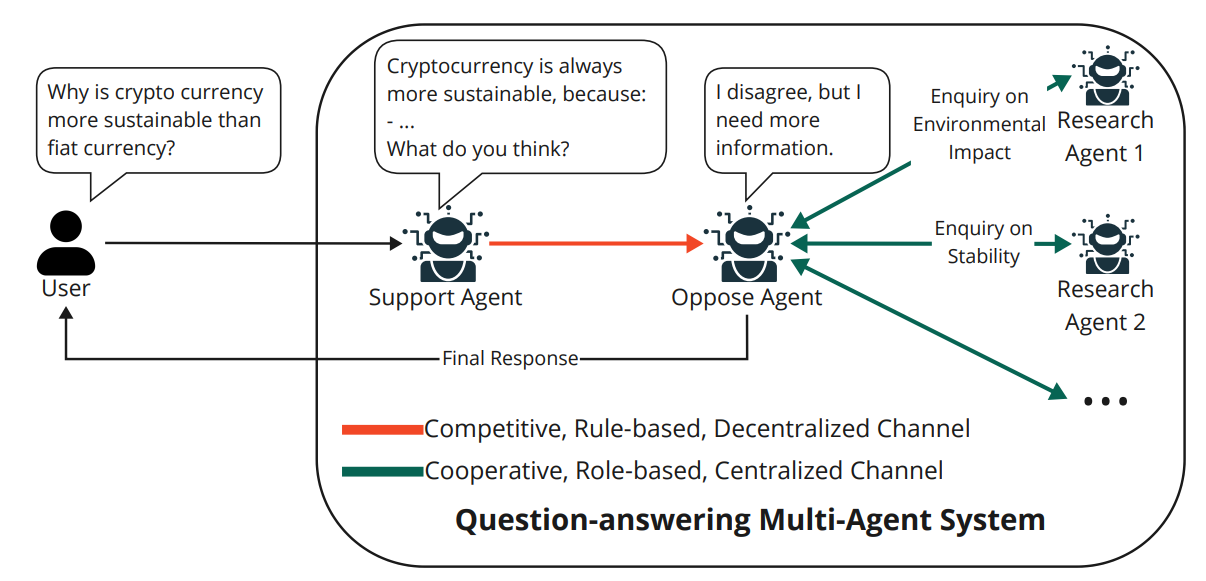
\includegraphics[width=0.9\textwidth]{Bilder/NLP_Application.png}
        \caption{Illustration of a question-answering multi-agent system as an example of agent collaboration and competition. Specialized agents interact through two communication channels: a competitive, rule-based, decentralized channel (red) and a cooperative, role-based, centralized channel (green), producing a final response to the user query \cite{tran2025multiagentcollaborationmechanismssurvey}.}
        \label{fig:NLP_Application}
    \end{figure}
    \FloatBarrier